\documentclass[aspectratio=169]{beamer}
\usetheme{BMW}

\usepackage{tikz}
\usetikzlibrary{shadows}

\usepackage{mflogo}

\usepackage{listings}
\lstdefinelanguage{TRLC}{
  keywords = {abs, and, checks, enum, error, extends, false, fatal, forall, implies, import, in, not, null, optional, or, package, section, true, type, warning, xor},
  comment=[l]{//},
  morecomment=[s]{/*}{*/},
  showstringspaces=false,
  string=[b]{"},
  delim=[s][stringstyle]{'''}{'''}
}
\lstset{language=TRLC}

\lstdefinestyle{smallstyle}
   {basicstyle=\scriptsize\tt,
    keywordstyle=\color{structure},
    commentstyle=\rmfamily\it\color{black!40},
    stringstyle=\color{brown!50!black},
    captionpos=b,
    caption={},label={},
    numbers=none,
    escapeinside={(*}{*)}}
  \lstset{style=smallstyle}

\newcommand{\email}[1]{\href{mailto:#1}{\structure{#1}}}

\classificationPublic
\author{Stefan Schlichthaerle, Philipp Wullstein-Kammler, Florian Schanda}
%\department{JC-12}
\title{Treat Requirements Like Code}
\date{February 20, 2023}

\begin{document}
\maketitle

\section{Contents}
\begin{frame}{Contents}
  \begin{itemize}
  \item The problem: why are we doing this
  \item Our requirements language
  \item Our traceability approach
  \item The holy grail: atomic commits
  \end{itemize}
\end{frame}

\section{The problem}
\begin{frame}{Context}
  \begin{itemize}
  \item Requirements are important
  \item We have more than $100,000$ requirements
  \item Traditional approach in the automotive industry is to use
    requirement management tools
  \end{itemize}
  \begin{center}
    \begin{tikzpicture}
      \node[drop shadow,inner sep=0,rotate=5] at (0,0)
      {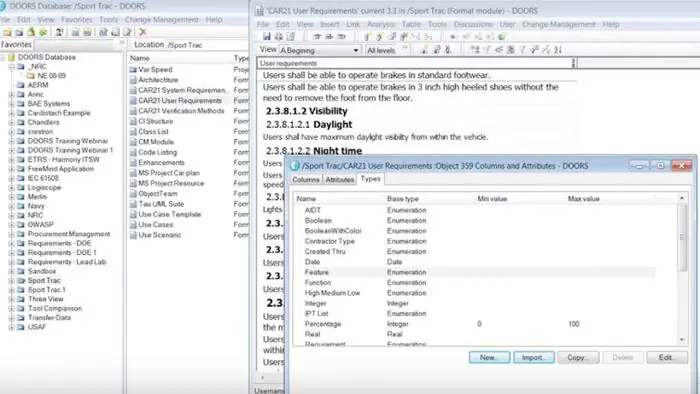
\includegraphics[width=5cm]{pictures/doors.png}};

      \node[drop shadow,inner sep=0,rotate=-20] at (3,1)
      {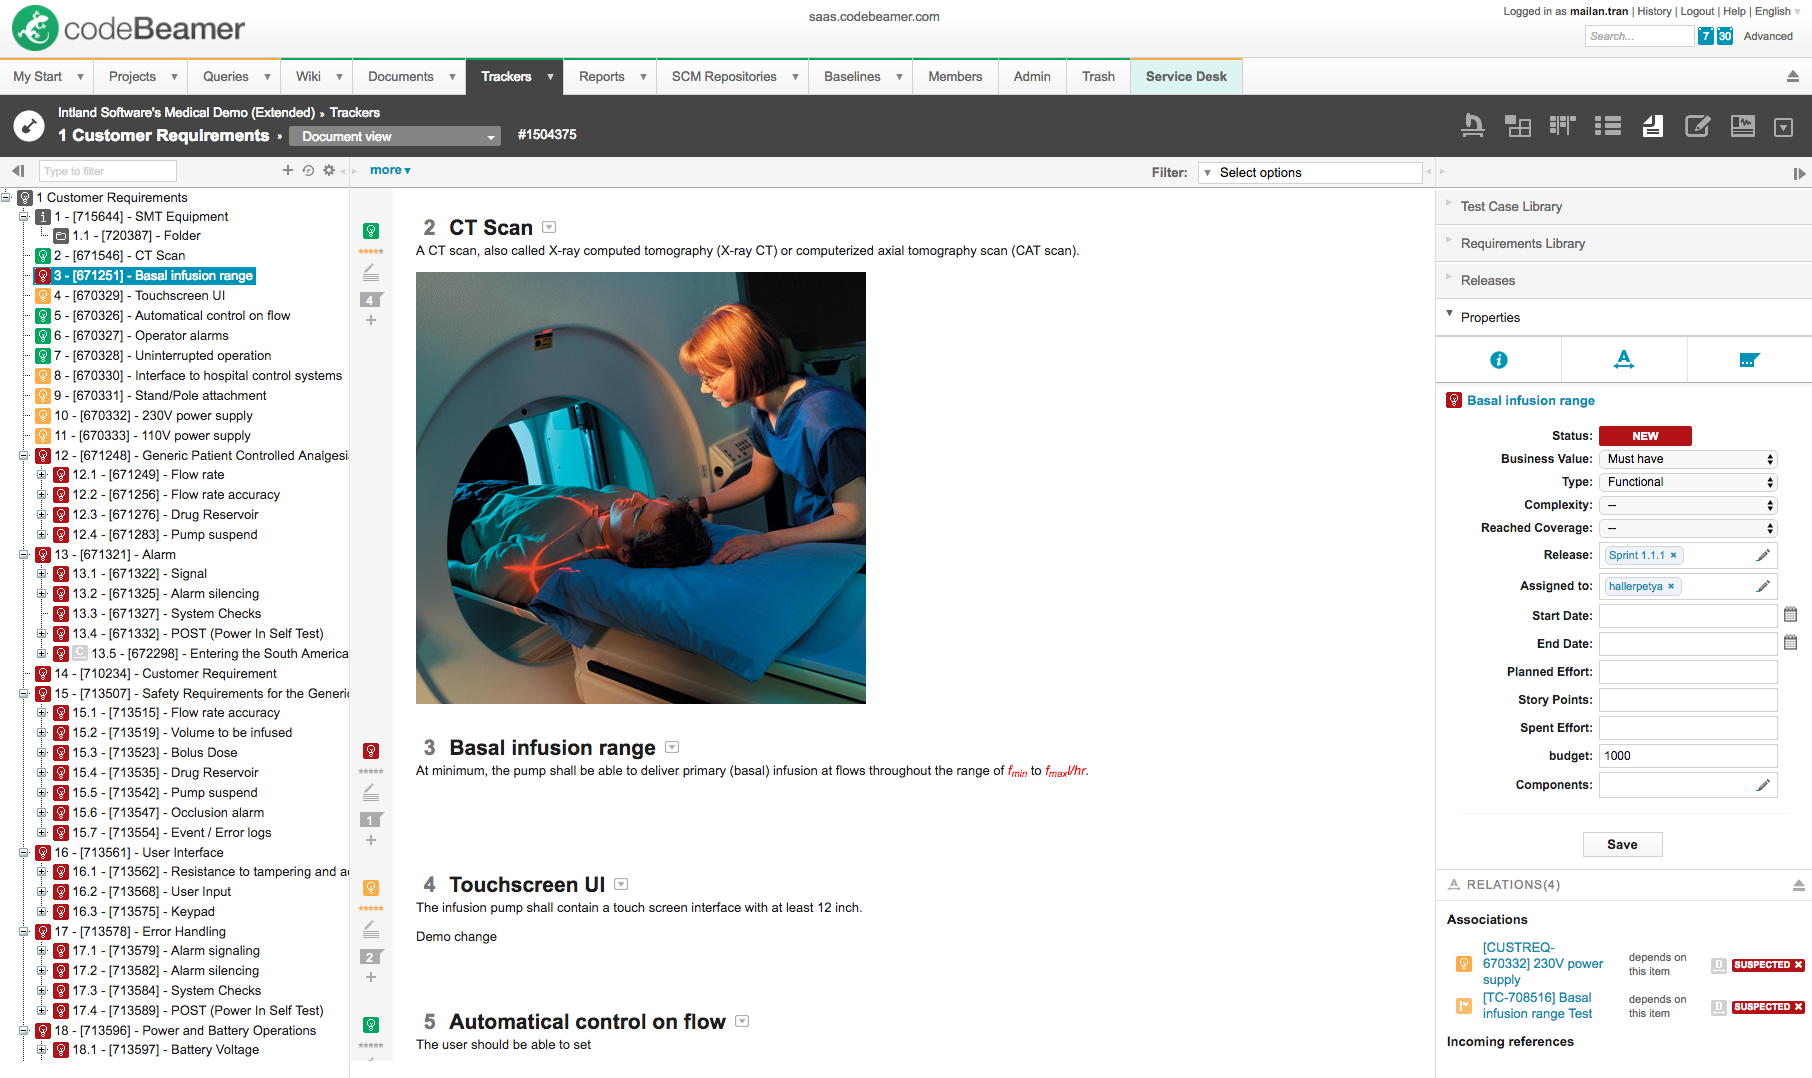
\includegraphics[width=5cm]{pictures/codebeamer.png}};

      \node[drop shadow,inner sep=0,rotate=10] at (-3,1)
      {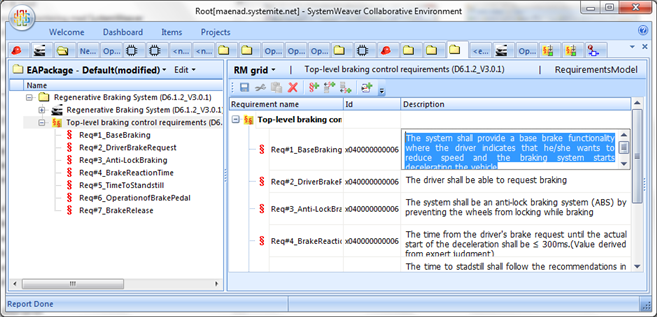
\includegraphics[width=5cm]{pictures/systemweaver.png}};
    \end{tikzpicture}
  \end{center}
\end{frame}

\begin{frame}{Common problems}
  Everyone should recognise at least some of these:
  \begin{itemize}
  \item Branching and version control is painful
  \item Tracability is extremely painful
  \item Releasing / updating requirements is painful
  \item Diffing and review is painful
  \item Duplication of information (e.g. mirroring tests in your
    favourite tool)
  \item Vendor lock-in
  \item Developers hate it
  \end{itemize}
\end{frame}

\begin{frame}{Root cause}{Our hypothesis}
  \begin{itemize}
  \item Disconnection from the actual artefact is the problem
  \item Representing requirements in the same (git) repository solves
    a lot of problems
  \end{itemize}
\end{frame}

\begin{frame}{Other approaches}{Requirement in code?}
  Requirements $\neq$ API documentation
  \begin{itemize}
  \item ``Just use doxygen'' is not the answer for this problem
  \item Requirements don't correspond 1:1 with source functions
  \item Requirements have levels, and need linking
  \item Requirements need additional meta-data
  \item Requirements need to be easily exported to other formats
  \end{itemize}
\end{frame}

% \begin{frame}{Other approaches}{Requirements are code?}
%   Literate programming could be an answer:
%   \begin{itemize}
%   \item First proposed by Knuth for \MF{}
%   \item Write documentation with embedded code
%   \item Compilation first extracts code, then compiles normally
%     \pause
%   \item Code generation from models or formal languages is somewhat
%     similar
%     \pause
%   \item However: this is \structure{too far away} from what most
%     people are used to
%   \end{itemize}
% \end{frame}

\section{TRLC}
\subsection{Overview}
\begin{frame}{Our approach \& design goals}
  \begin{itemize}
  \item Keep requirements in plain text separate, but close, to the code
    \begin{itemize}
    \item Solves the version control problem
    \item Solves the diffing, branching, and merging problems
    \item Solves the updating and releasing problems
    \end{itemize}
    \pause

  \item Keep it open and machine parseable
    \begin{itemize}
    \item Contributes to solving the tracing problem
    \item No more vendor lock-in
    \end{itemize}
    \pause

  \item Don't bake in policy
    \begin{itemize}
    \item Policy changes, this should not require tool changes
    \item Other companies don't have our policy
    \end{itemize}
  \end{itemize}
\end{frame}

\begin{frame}{TRLC}
  \structure{T}reat \structure{R}equirements \structure{L}ike \structure{C}ode\\
  \url{https://github.com/bmw-software-engineering/trlc} (GPL v3)
  \begin{itemize}
  \item Plain text carrier format with meta-data, linking, and
    user-defined policy
  \item Define types and checks (policy) in \texttt{.rsl} files
  \item Define requirements in \texttt{.trlc} files
  \item Python API to write clever tools
  \end{itemize}
\end{frame}

\subsection{Example}
\begin{frame}[fragile]{Example}{Types}
  \begin{lstlisting}
enum ASIL { QM A B C D }

type Requirement {
    description String

    asil        optional ASIL
    test_method optional TestMethod
    sotif       optional SOTIF
    security    optional Security
    attachments optional String [0..*]

    derived_from_cb         optional Integer     [0..*]
    derived_from_trlc       optional Requirement [0..*]
}

type Constant {
    description String
    value       Integer
    unit        String
}
  \end{lstlisting}
\end{frame}

\begin{frame}[fragile]{Example}{Policy}
  \begin{lstlisting}[gobble=4]
    checks Requirement {
      len(description) >= 10,
        "The description must have at least 10 characters."

      derived_from_cb != null or derived_from_trlc != null,
        warning "At least one upstream reference should be given
          to a parent requirement in either codebeamer or TRLC."

      attachments != null implies
        (forall filename in attachments => len(filename) >= 1),
        warning "please write more"
    }
  \end{lstlisting}
\end{frame}

\begin{frame}[fragile]{Example}{Requirement}
  \begin{lstlisting}[gobble=4]
    Requirement potato {
      description = "This is an example"

      asil = ASIL.B_of_D
      attachments = ["assets/potato.png"]
    }
  \end{lstlisting}
  \pause
  \begin{block}{TRLC tool output}
    \scriptsize
\begin{verbatim}
Requirement potato {
            ^^^^^^ potato.trlc:3: check warning: At least one upstream reference should be
                   given to a parent requirement in either codebeamer or TRLC.
\end{verbatim}
  \end{block}
\end{frame}

\subsection{Use-case: TRLC LRM}
\begin{frame}{Machine parsing for the win}
  Ability to process requirements and metadata in a Python API enables
  all sorts of interesting use-cases...
\end{frame}

\begin{frame}[fragile]{Use-case: TRLC LRM}
  The language reference manual for TRLC will be in TRLC:
  \begin{lstlisting}
section "Preamble" {

  Grammar Preamble {
    text = "All TRLC files start with a package indication."
    bnf = '''
      file_preamble ::= package_indication
                        { import_clause }

      package_indication ::= 'package' IDENTIFIER_name

      import_clause ::= 'import' IDENTIFIER_name
      '''
  }

  Semantics Current_Package {
    kind = Kind.Static
    text = '''The package indication defines the "current package".'''
  }
  \end{lstlisting}
  \pause
  \begin{tikzpicture}[remember picture,overlay]
    \node[inner sep=0] at (10,4) {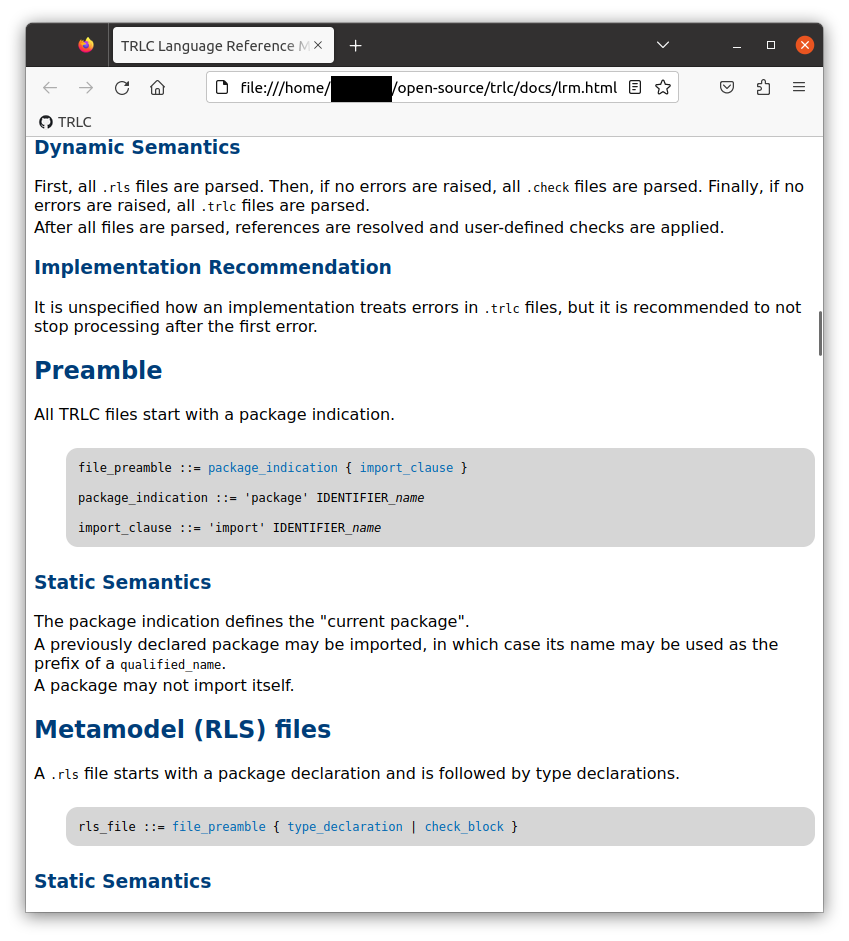
\includegraphics[width=8cm]{pictures/lrm}};
  \end{tikzpicture}
\end{frame}

\subsection{Use-case: Formal methods}
\begin{frame}[fragile]{Use-case: More formality?}
  \begin{lstlisting}[gobble=4]
    ZSchema AdvanceTimer {
      asil = ASIL.D
      declarations = ["\Delta Timer",
                      "timeIncrement? : TIME"]
      predicates   = ["0 \leq timeIncrement?",
                      "limit' = limit",
                      "time' = min(time + timeIncrement?, limit)"]
      description = '''
        To advance the timer by $timeIncrement?$ we simply add
        this to $time$, up to the $limit$ configured in the timer.
        The timer's $limit$ is not changed.
      '''
    }
  \end{lstlisting}
  \pause
  \begin{tikzpicture}[remember picture,overlay]
    \node[fill=white,drop shadow,rotate=10,draw] at (11, 3) {
      \includegraphics[width=8cm]{pictures/schema.pdf}
    };
  \end{tikzpicture}
  \begin{itemize}
  \item Generate PDF document
    \pause
  \item Generate Z fragment for type checking with fuzz
  \item Generate SMTLIB2 for automatic model checking?
  \item Generate SPARK contracts for formal program proof?
  \end{itemize}
\end{frame}

\section{Tracability}
\begin{frame}{Tracability}
  One big unsolved issue:
  \begin{itemize}
  \item Did I cover all my requirements? Are there gaps?
  \item Why does this code exist?
  \item How does it all relate?
  \item Often this is a manual and painful activity
    \begin{itemize}
    \item Tests need to be imported: duplication of information is bad
    \item Code tracing never happens
    \item Adding a new language/tool breaks everything
    \end{itemize}
  \end{itemize}
\end{frame}

\begin{frame}{LOBSTER}
  \structure{L}ightweight \structure{O}pen \structure{B}MW
  \structure{S}oftware \structure{T}raceability \structure{E}vidence
  \structure{R}eport\\
  \url{https://github.com/bmw-software-engineering/lobster} (AGPL v3)
  \begin{itemize}
  \item Generic format to represent traceable items
  \item One tool to link everything together
  \end{itemize}
\end{frame}

\begin{frame}[fragile]{LOBSTER}{Tracing tags}
  For example in C++ code:
  \begin{lstlisting}[language=c++,gobble=4]
    int implication(int x, int y)
    {
      // lobster-trace: example.req_implication
      return (x == 0) || (y != 0);
    }
  \end{lstlisting}

  Or in googletest unit tests:
  \begin{lstlisting}[language=c++,gobble=4]
    TEST(ImplicationTest, BasicTest)
    {
      LOBSTER_TRACING("example.req_implication");

      EXPECT_TRUE(implication(false, true));
      EXPECT_TRUE(implication(true, true));
    }
  \end{lstlisting}
\end{frame}

\begin{frame}{LOBSTER}{Report}
  \begin{center}
    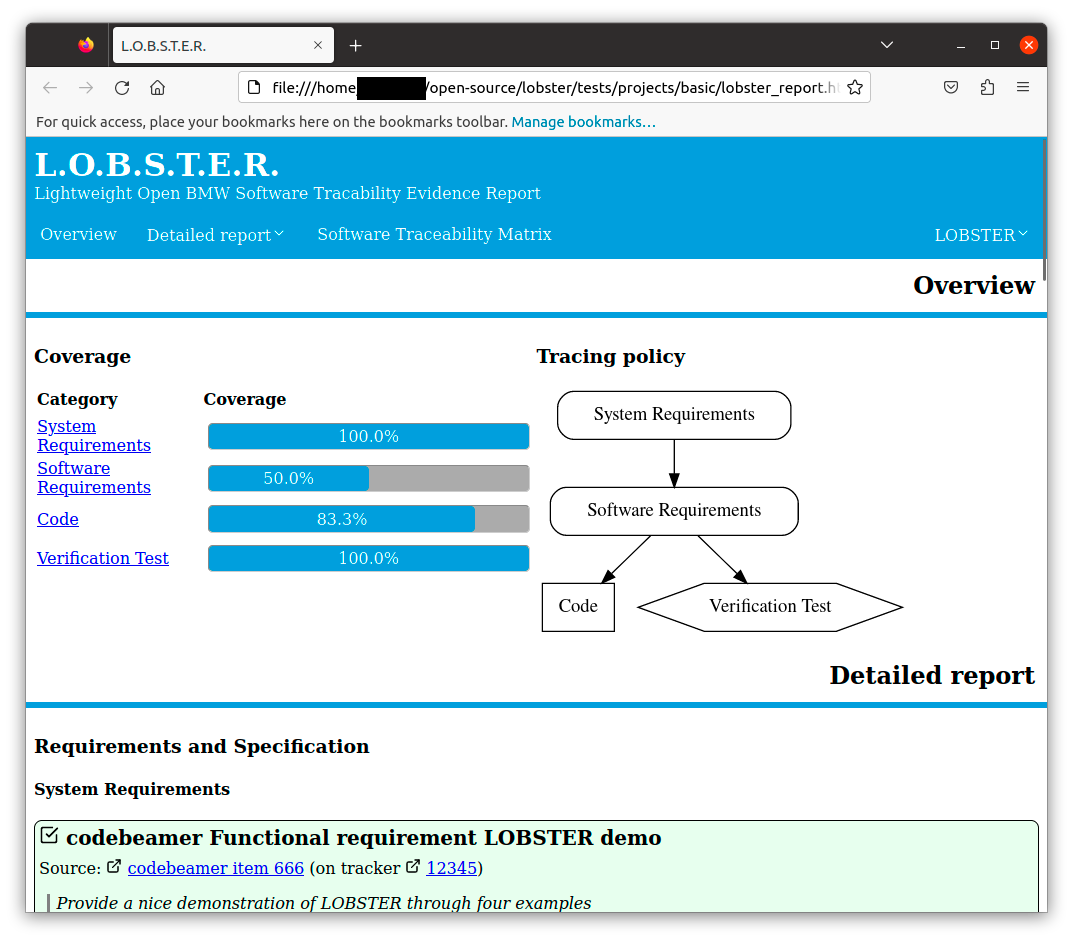
\includegraphics[height=0.8\textheight]{pictures/lobster.png}
  \end{center}
\end{frame}

\begin{frame}[fragile]{LOBSTER}{CI Integration}
  We can check everything in CI as well and block merges:
  \scriptsize
\begin{verbatim}
potato.trlc:21: tracing error on example.req_nor: missing reference to Verification Test
potato.trlc:9: tracing error on example.req_xor: missing reference to Code
potato.trlc:9: tracing error on example.req_xor: missing reference to Verification Test
foo.cpp:9: tracing error on exclusive_or:9: missing up reference
\end{verbatim}
\end{frame}

\begin{frame}{LOBSTER}{Tracing tags}
  \begin{columns}
    \begin{column}{0.5\textwidth}
      Support exists for:
      \begin{itemize}
      \item C, C++ (via a custom clang-tidy plugin)
      \item MATLAB, Simulink (via MISS\_HIT)
      \item Python
      \item googletest (through parsing the XML output file)
      \item TRLC
      \end{itemize}
    \end{column}
    \begin{column}{0.5\textwidth}
      Planned / in the works:
      \begin{itemize}
      \item Java
      \item Kotlin
      \item Ada and SPARK
      \item Rust
      \item Z, TLA+
      \item codebeamer
      \end{itemize}
    \end{column}
  \end{columns}

  \pause
  \vspace{1cm}
  Note: it's trivial to add support for your own custom tools /
  environments / methods.
\end{frame}

\section{The Holy Grail}
\begin{frame}{Atomic commits}{The holy grail}
  \begin{itemize}
  \item One commit has:
    \begin{itemize}
    \item requirements change
    \item code change
    \item verification and validation change
    \item tracaebility argument
    \end{itemize}
  \item Which requirement belong to which code: obvious (same git revision)
  \item Tracing argument: obvious (not possible to merge otherwise)
  \item Branching: just do it in git
  \item Merging: just do it in git
  \item Diffing: do it in your favourite diff tool
  \item Reviewing: gerrit/github/gitlab
  \end{itemize}
\end{frame}

\section{Conclusion}
\begin{frame}{Future work \& Conclusion}
  \begin{itemize}
  \item Developers \structure{love} it, and we already use this in
    many projects
  \item Generate internal metrics on how much time this really saves,
    and convince everyone else
    \pause
  \item Build an open-source community around TRLC and LOBSTER
  \item New features based on internal and external feedback
    \pause
  \item Tool qualification up to ASIL-D
  \end{itemize}
  \pause
  \begin{center}
    \url{https://github.com/bmw-software-engineering}
  \end{center}
  \pause
  \hrule
  \begin{center}
    {\Large\bf We're hiring!}\\
    Contact \email{florian.schanda@bmw.de}~or
    \email{philipp.wullstein-kammler@bmw.de}
  \end{center}
  \pause
  \hrule
  \begin{center}
    Thank you for listening.\\
    \structure{Questions?}
  \end{center}
\end{frame}

\end{document}
